\documentclass{ximera}  

\title{Vectors}  

\begin{document}  
\begin{abstract}  
%abstract
\end{abstract}  
\maketitle 

In this section, we review some basics about vectors. This includes the definition of a vector, basic vector operations, standard basis vectors, and notation.

\section{Vectors}

In linear algebra, we often worked with vectors. We begin by recalling the (algebraic) definition of a vector in $\mathbb{R}^n$.

\begin{definition}
A \emph{vector} in $\mathbb{R}^n$ is an ordered $n$-tuple of real numbers. That is, a vector $\vec{v}$ may be written as
\[
\vec{v} = (a_1,a_2,...,a_n)
\]
where $a_1,a_2,...,a_n$ are real numbers.

We call the numbers $a_i$ the \emph{components} or \emph{entries} of the vector. We call $n$ the \emph{dimension} of the vector $\vec{v}$, and say that $\vec{v}$ is \emph{$n$-dimensional}.
\end{definition}

We write the vector with an arrow above it, as $\vec{v}$, in order to make the distinction between vectors and \emph{scalars}, which are just real numbers. Some other common notations for vectors are $\mathbf{v}$ and $\hat{v}$. It's important to make this distinction between vectors and scalars, so you should make use of one of these notations for vectors.

\begin{example}
$\vec{v} = (1,3)$ is a vector in $\mathbb{R}^2$.

$\vec{w} = (-1,5,0)$ is a vector in $\mathbb{R}^3$.

$\vec{x} = (1,-2,3)$ is a vector in $\mathbb{R}^3$.

$\vec{y} = (-6,\pi, 1/24, -0.5, 3)$ is a vector in $\mathbb{R}^5$.
\end{example}

It's sometimes convenient to write a vector as a column vector instead (particularly when working with linear transformations, which we'll review in a later section). We could write
\[
\vec{v} = (a_1,a_2,...,a_n)=\left[\begin{array}{c}a_1\\a_2\\\vdots\\a_n\end{array}\right]
\]
or
\[
\vec{v} = (a_1,a_2,...,a_n)=\left(\begin{array}{c}a_1\\a_2\\\vdots\\a_n\end{array}\right).
\]
The choice between square brackets and parentheses is just a difference in notation, they mean the same thing, and you should feel free to use either.

\begin{example}
We write the following vectors as column vectors.

$\vec{v} = (1,3)=\left[\begin{array}{c}1\\3\end{array}\right]$.

$\vec{w} = (-1,5,0)=\left[\begin{array}{c}-1\\5\\0\end{array}\right]$.

$\vec{x} = (1,-2,3)=\left[\begin{array}{c}1\\-2\\3\end{array}\right]$.

$\vec{y} = (-6,\pi, 1/24, -0.5, 3)=\left[\begin{array}{c}-6\\\pi\\1/24\\-0.5\\3\end{array}\right]$.
\end{example}

\section{The Geometric Perspective}

We also can think of a vector geometrically, as giving a direction and magnitude, but without a fixed position.

In two or three dimensions, it is useful to visualize a vector as an arrow in $\mathbb{R}^n$. We might visualize a vector $\vec{v}=(1,3)$ in $\mathbb{R}^2$ as the arrow starting at the origin and ending at the point $(1,3)$, thus giving a direction and a magnitude. However, we typically don't think of a vector as having a set location. We could also visualize the vector $\vec{v}$ as starting at the point $(-1,-1)$ and ending at the point $(0,2)$. Note that this arrow would have the same direction and magnitude as the one starting at the origin, thus they represent the same vector.

\begin{image}
\begin{tikzpicture}
\draw[<->] (-1,0) -- (2,0);
\draw[<->] (0,-1) -- (0,4);
\foreach \x in  {0,1}
\draw[shift={(\x,0)},color=black] (0pt,3pt) -- (0pt,-3pt);
\foreach \x in {0,1}
\draw[shift={(\x,0)},color=black] (0pt,0pt) -- (0pt,-3pt) node[below] 
{$\x$};
\foreach \y in  {0,3}
\draw[shift={(0,\y)},color=black] (3pt,0pt) -- (-3pt,0pt);
\foreach \y in {0,3}
\draw[shift={(0,\y)},color=black] (0pt,0pt) -- (-3pt,0pt) node[left] 
{$\y$};

\node[draw, circle, thick, fill=black, minimum size=1mm, inner sep=0] at (0,0) {};
\draw[->, very thick] (0,0) -- (1,3);

\begin{scope}[xshift=6cm, yshift = 1cm]

\draw[<->] (-2,0) -- (1,0);
\draw[<->] (0,-2) -- (0,3);
\foreach \x in  {-1,0}
\draw[shift={(\x,0)},color=black] (0pt,3pt) -- (0pt,-3pt);
\foreach \x in {-1,0}
\draw[shift={(\x,0)},color=black] (0pt,0pt) -- (0pt,-3pt) node[below] 
{$\x$};
\foreach \y in  {-1,0,2}
\draw[shift={(0,\y)},color=black] (3pt,0pt) -- (-3pt,0pt);
\foreach \y in {-1,0,2}
\draw[shift={(0,\y)},color=black] (0pt,0pt) -- (-3pt,0pt) node[left] 
{$\y$};

\node[draw, circle, thick, fill=black, minimum size=1mm, inner sep=0] at (-1,-1) {};
\draw[->, very thick] (-1,-1) -- (0,2);

\end{scope}
\end{tikzpicture}
\end{image}

In four or higher dimensions, visualizing anything becomes very difficult. It can still be useful to think of a vector $(1,2,3,4,5)$ in $\mathbb{R}^5$ as starting at the origin and ending at the point $(1,2,3,4,5)$, but you probably won't be able to have a very clear picture of this in your head.

This concept will probably seem more useful once you think about a displacement vector.

\begin{definition}
Given points $P_1 = (x_1,...,x_n)$ and $P_2 = (y_1,...,y_n)$ in $\mathbb{R}^n$, the \emph{displacement vector} from $P_1$ to $P_2$ is
\[
\vec{P_1P_2} = (y_1 - x_1,..., y_n - x_n).
\]
This is the vector that starts at $P_1$ and ends at $P_2$.
\end{definition}

Notice that the notation $(a_1,...,a_n)$ that we use for a vector in $\mathbb{R}^n$ is identical to the notation that we'd use for a point in $\mathbb{R}^n$. Since both vectors and points in $\mathbb{R}^n$ are defined as $n$-tuples of points, they are, in some sense, the same thing. The difference between the two comes when we consider the context and geometric significance of the vector or point that we're working with. As we move into multivariable calculus, we'll often blur the distinction between a vector and a point, and sometimes think of a vector as a point and vice versa. This will be greatly simplify notation, and we promise that it won't be as confusing as it sounds!

\section{Vector Operations}

Before defining some basic vector operations, we define what it means for two vectors to be equal. This is done by comparing the components of the vectors.

\begin{definition}
Two vectors $(a_1,a_2,...,a_n)$ and $(b_1,b_2,...,b_n)$ in $\mathbb{R}^n$ are \emph{equal} if their corresponding components are equal, so $a_1=b_1$, $a_2=b_2$, ... , $a_n = b_n$.
\end{definition}

Notice that, in order to be equal, two vectors must have the same dimension and the same entries in the same order. Thus, the vectors $(1,3)$ and $(1,3,0)$ are not equal.

We now define addition of two vectors of the same dimension, which is done componentwise.

\begin{definition}
Let $\vec{a}=(a_1,a_2,...,a_n)$ and $\vec{b}=(b_1,b_2,...,b_n)$ be vectors in $\mathbb{R}^n$. We define $\vec{a}+\vec{b}$ to be the vector in $\mathbb{R}^n$ given by
\[
\vec{a}+\vec{b} = (a_1+b_1,a_2+b_2,...,a_n+b_n).
\]
\end{definition}

Note that we can only add two vectors if they have the same dimension.

\begin{example}
Adding the vectors $\vec{a} = (1,-8,2)$ and $\vec{b} = (3,-1,-2)$, we obtain
\begin{align*}
\vec{a}+\vec{b} &= (1,-8,2)+(3,-1,-2)\\
 &= (1+3,-8-1,2-2)\\
 &= (4,-9,0).
\end{align*}
\end{example}

Geometrically, we can add vectors by placing the start point of the second vector at the end point of the first vector, and drawing an arrow from the start point of the first vector to the end point of the second vector.

\begin{example}
In this example, we add the vectors $(1,1)$ and $(1,3)$. Adding these vectors algebraically, we obtain $(2,4)$. We can also see this geometrically by placing the start point of the vector $(1,3)$ at the end of the vector $(1,1)$ (so at the point $(1,1)$), and drawing the vector from the origin to the end point of the vector $(1,3)$, which is now at $(2,4)$.

\begin{image}
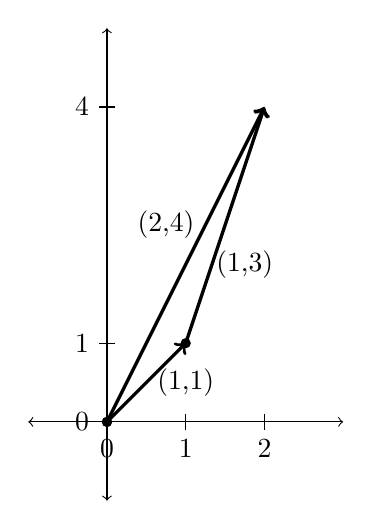
\begin{tikzpicture}
\draw[<->] (-1,0) -- (3,0);
\draw[<->] (0,-1) -- (0,5);
\foreach \x in  {0,1,2}
\draw[shift={(\x,0)},color=black] (0pt,3pt) -- (0pt,-3pt);
\foreach \x in {0,1,2}
\draw[shift={(\x,0)},color=black] (0pt,0pt) -- (0pt,-3pt) node[below] 
{$\x$};
\foreach \y in  {0,1,4}
\draw[shift={(0,\y)},color=black] (3pt,0pt) -- (-3pt,0pt);
\foreach \y in {0,1,4}
\draw[shift={(0,\y)},color=black] (0pt,0pt) -- (-3pt,0pt) node[left] 
{$\y$};

\node[draw, circle, thick, fill=black, minimum size=1mm, inner sep=0] at (0,0) {};
\draw[->, very thick] (0,0) -- (1,1);

\node[draw, circle, thick, fill=black, minimum size=1mm, inner sep=0] at (1,1) {};
\draw[->, very thick] (1,1) -- (2,4);


\node[draw, circle, thick, fill=black, minimum size=1mm, inner sep=0] at (0,0) {};
\draw[->, very thick] (0,0) -- (2,4);

\node at (1, 0.5) {(1,1)};
\node at (1.75, 2) {(1,3)};
\node at (0.75, 2.5) {(2,4)};

\end{tikzpicture}
\end{image}
\end{example}

Another vector operation is scalar multiplication. Here, we multiply a vector by a real number, possibly changing the length of the vector.

\begin{definition}
Let $\vec{a}=(a_1,...,a_n)$ be a vector in $\mathbb{R}^n$, and let $r$ be a real number (also called a scalar). We define the \emph{scalar product} $r\vec{a}$ to be
\[
r\vec{a} = (ra_1,...,ra_n).
\]
\end{definition}

Thus, we see that scalar multiplication is defined by multiplying each component of the vector by the scalar $r$.

\begin{example}
$3(1,5,-2)=(3,15,-6)$

$-1(1,1,1)=(-1,-1,-1)$

$0(6,2,4) = (0,0,0)$
\end{example}

Now, let's look at what scalar multiplication does geometrically. Consider the vector $(1,3)$. 

When we multiply $(1,3)$ by $2$, we obtain $(2,6)$, which is twice as long as $(1,3)$ and goes in the same direction.

\begin{image}
\begin{tikzpicture}
\draw[<->] (-1,0) -- (7,0);
\draw[<->] (0,-1) -- (0,7);
\foreach \x in  {0,1}
\draw[shift={(\x,0)},color=black] (0pt,3pt) -- (0pt,-3pt);
\foreach \x in {0,1}
\draw[shift={(\x,0)},color=black] (0pt,0pt) -- (0pt,-3pt) node[below] 
{$\x$};
\foreach \y in  {0,3}
\draw[shift={(0,\y)},color=black] (3pt,0pt) -- (-3pt,0pt);
\foreach \y in {0,3}
\draw[shift={(0,\y)},color=black] (0pt,0pt) -- (-3pt,0pt) node[left] 
{$\y$};

\node[draw, circle, thick, fill=black, minimum size=1mm, inner sep=0] at (0,0) {};
\draw[->, very thick] (0,0) -- (1,3);
\node at (1.5,3) {$(1,3)$};

\begin{scope}[xshift=10cm]

\draw[<->] (-1,0) -- (7,0);
\draw[<->] (0,-1) -- (0,7);
\foreach \x in  {0,1}
\draw[shift={(\x,0)},color=black] (0pt,3pt) -- (0pt,-3pt);
\foreach \x in {0,1}
\draw[shift={(\x,0)},color=black] (0pt,0pt) -- (0pt,-3pt) node[below] 
{$\x$};
\foreach \y in  {0,3}
\draw[shift={(0,\y)},color=black] (3pt,0pt) -- (-3pt,0pt);
\foreach \y in {0,3}
\draw[shift={(0,\y)},color=black] (0pt,0pt) -- (-3pt,0pt) node[left] 
{$\y$};

\node[draw, circle, thick, fill=black, minimum size=1mm, inner sep=0] at (0,0) {};
\draw[->, very thick] (0,0) -- (2,6);
\node at (2.5,6) {$(2,6)$};

\end{scope}
\end{tikzpicture}
\end{image}

 When we multiply $(1,3)$ by $\frac{1}{2}$, we obtain $\left(\frac{1}{2},\frac{3}{2}\right)$, which is half as long as $(1,3)$ and goes in the same direction. 
 
 \begin{image}
\begin{tikzpicture}
\draw[<->] (-1,0) -- (4,0);
\draw[<->] (0,-1) -- (0,4);
\foreach \x in  {0,1}
\draw[shift={(\x,0)},color=black] (0pt,3pt) -- (0pt,-3pt);
\foreach \x in {0,1}
\draw[shift={(\x,0)},color=black] (0pt,0pt) -- (0pt,-3pt) node[below] 
{$\x$};
\foreach \y in  {0,3}
\draw[shift={(0,\y)},color=black] (3pt,0pt) -- (-3pt,0pt);
\foreach \y in {0,3}
\draw[shift={(0,\y)},color=black] (0pt,0pt) -- (-3pt,0pt) node[left] 
{$\y$};

\node[draw, circle, thick, fill=black, minimum size=1mm, inner sep=0] at (0,0) {};
\draw[->, very thick] (0,0) -- (1,3);
\node at (1.5,3) {$(1,3)$};

\begin{scope}[xshift=10cm]

\draw[<->] (-1,0) -- (4,0);
\draw[<->] (0,-1) -- (0,4);
\foreach \x in  {0,1}
\draw[shift={(\x,0)},color=black] (0pt,3pt) -- (0pt,-3pt);
\foreach \x in {0,1}
\draw[shift={(\x,0)},color=black] (0pt,0pt) -- (0pt,-3pt) node[below] 
{$\x$};
\foreach \y in  {0,3}
\draw[shift={(0,\y)},color=black] (3pt,0pt) -- (-3pt,0pt);
\foreach \y in {0,3}
\draw[shift={(0,\y)},color=black] (0pt,0pt) -- (-3pt,0pt) node[left] 
{$\y$};

\node[draw, circle, thick, fill=black, minimum size=1mm, inner sep=0] at (0,0) {};
\draw[->, very thick] (0,0) -- (0.5,1.5);
\node at (1.25,1.5) {$\left(\frac{1}{2},\frac{3}{2}\right)$};

\end{scope}
\end{tikzpicture}
\end{image}
 
 If we multiply $(1,3)$ by $-2$, we obtain $(-2,-6)$, which is twice as long as $(1,3)$ and goes in the exact opposite direction.
 
  \begin{image}
\begin{tikzpicture}
\draw[<->] (-7,0) -- (4,0);
\draw[<->] (0,-7) -- (0,4);
\foreach \x in  {0,1}
\draw[shift={(\x,0)},color=black] (0pt,3pt) -- (0pt,-3pt);
\foreach \x in {0,1}
\draw[shift={(\x,0)},color=black] (0pt,0pt) -- (0pt,-3pt) node[below] 
{$\x$};
\foreach \y in  {0,3}
\draw[shift={(0,\y)},color=black] (3pt,0pt) -- (-3pt,0pt);
\foreach \y in {0,3}
\draw[shift={(0,\y)},color=black] (0pt,0pt) -- (-3pt,0pt) node[left] 
{$\y$};

\node[draw, circle, thick, fill=black, minimum size=1mm, inner sep=0] at (0,0) {};
\draw[->, very thick] (0,0) -- (1,3);
\node at (1.5,3) {$(1,3)$};

\begin{scope}[xshift=10cm]

\draw[<->] (-7,0) -- (4,0);
\draw[<->] (0,-7) -- (0,4);
\foreach \x in  {0,1}
\draw[shift={(\x,0)},color=black] (0pt,3pt) -- (0pt,-3pt);
\foreach \x in {0,1}
\draw[shift={(\x,0)},color=black] (0pt,0pt) -- (0pt,-3pt) node[below] 
{$\x$};
\foreach \y in  {0,3}
\draw[shift={(0,\y)},color=black] (3pt,0pt) -- (-3pt,0pt);
\foreach \y in {0,3}
\draw[shift={(0,\y)},color=black] (0pt,0pt) -- (-3pt,0pt) node[left] 
{$\y$};

\node[draw, circle, thick, fill=black, minimum size=1mm, inner sep=0] at (0,0) {};
\draw[->, very thick] (0,0) -- (-2,-6);
\node at (-0.75,-5) {$(-2,-6)$};

\end{scope}
\end{tikzpicture}
\end{image}
 
Thus, we have seen that multiplying a vector by a scalar changes the length of a vector, but not the direction (except for reversing it, if the scalar is negative). 

\section{Properties}

Now, let's recall some useful properties of vector addition and scalar multiplication.

\begin{proposition}
Suppose $\vec{a},\vec{b},\vec{c}$ are vectors in $\mathbb{R}^n$ and $k,l$ are real numbers. Then 
\begin{enumerate}
\item $\vec{a}+\vec{b} = \vec{b}+\vec{a}$ (vector addition is \emph{commutative});
\item $\vec{a}+(\vec{b}+\vec{c}) = (\vec{a}+\vec{b})+\vec{c}$ (vector addition is \emph{associative});
\item $\vec{a}+\vec{0} = \vec{0}+\vec{a} = \vec{a}$, where $\vec{0} = (0,...,0)$ is the \emph{zero vector} in $\mathbb{R}^n$;
\item $(k+l)\vec{a} = k\vec{a}+l\vec{a}$;
\item $k(\vec{a}+\vec{b}) = k\vec{a}+k\vec{b}$ (with the previous property, scalar multiplication is \emph{distributive});
\item $k(l\vec{a})=(kl)\vec{a} = l(k\vec{a})$;
\item $1\vec{a} = \vec{a}$.
\end{enumerate}
\end{proposition}

These properties tell us different kinds of algebraic manipulations that we can do with vectors.

\section{Standard Basis Vectors}

It's often useful to write things in terms of the standard basis vectors for $\mathbb{R}^n$.

\begin{definition}
The vectors $\vec{e}_1 = (1,0,...0)$, $\vec{e}_2 = (0,1,0,...,0)$, ..., $\vec{e}_n = (0,...,0,1)$ in $\mathbb{R}^n$ are called the \emph{standard basis vectors} for $\mathbb{R}^n$.
\end{definition}

Note that any vector in $\mathbb{R}^n$ can be written uniquely as a linear combination of the standard unit vectors. For example, in $\mathbb{R}^4$,
\begin{align*}
(1,5,-3,6) &= 1(1,0,0,0)+5(0,1,0,0)-3(0,0,1,0)+6(0,0,0,1)\\
&= 1\vec{e}_1+5\vec{e}_2-3\vec{e}_3+6\vec{e}_4.
\end{align*}

In $\mathbb{R}^2$, we sometimes write the standard basis vectors as $\mathbf{i} = (1,0)$ and $\mathbf{j} = (0,1)$. This gives us a new notation for vectors, for example we could write
\[
(3,4) = 3\mathbf{i}+4\mathbf{j}.
\]

Similarly, in $\mathbb{R}^3$, we sometimes write the standard basis vectors as $\mathbf{i} = (1,0,0)$, $\mathbf{j} = (0,1,0)$, and $\mathbf{k} = (0,0,1)$. We can then write
\[
(2,3,4) = 2\mathbf{i}+3\mathbf{j}+4\mathbf{k}.
\]

\section{Summary}

In this section, we reviewed some basics about vectors, including the definition of a vector, basic vector operations, standard basis vectors, notation, and the geometric perspective.

\end{document}